\documentclass[border=8pt]{standalone}
\usepackage{tikz}
\usepackage{mathptmx}
\usetikzlibrary{shadings, arrows.meta}
\definecolor{navy}{RGB}{20,52,110}
\definecolor{accent}{RGB}{14,110,120}
\definecolor{orange}{RGB}{200,110,30}
\definecolor{tcold}{RGB}{40,60,150}
\definecolor{tmid}{RGB}{40,150,140}
\definecolor{twarm}{RGB}{235,180,40}
\definecolor{thot}{RGB}{200,50,40}
\begin{document}
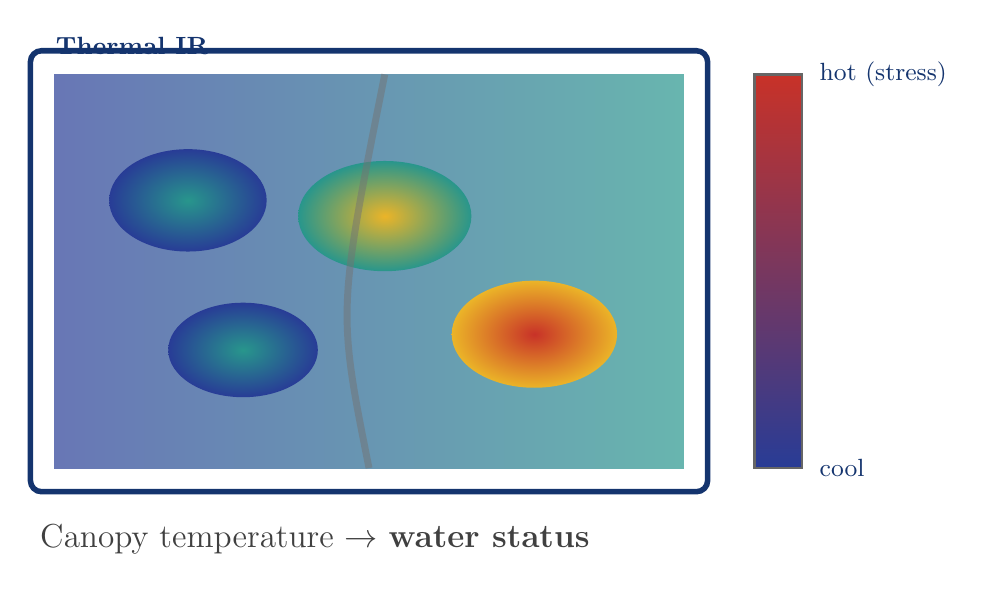
\begin{tikzpicture}[font=\sffamily]
% ---- thermal "camera" frame ----
\draw[line width=2pt, navy, rounded corners=4pt] (-0.3,-0.3) rectangle (8.3,5.3);
\node[anchor=north west, font=\small\bfseries, color=navy] at (-0.1,5.6) {Thermal IR};

% ---- background gradient (cool canopy) ----
\shade[left color=tcold!70, right color=tmid!70] (0,0) rectangle (8,5);

% ---- a few "leaf" blobs with hot/warm centres (stressed vs not) ----
% leaf 1 - cooler (well-watered)
\shade[inner color=tmid, outer color=tcold] (1.7,3.4) ellipse (1.0 and 0.65);
% leaf 2 - warm (mild stress)
\shade[inner color=twarm, outer color=tmid] (4.2,3.2) ellipse (1.1 and 0.7);
% leaf 3 - hot (water stress)
\shade[inner color=thot, outer color=twarm] (6.1,1.7) ellipse (1.05 and 0.68);
% leaf 4 - mid
\shade[inner color=tmid, outer color=tcold] (2.4,1.5) ellipse (0.95 and 0.6);

% stem hint
\draw[line width=2.5pt, black!55, opacity=0.5] (4,0) .. controls (3.6,2) .. (4.2,5);

% ---- colour-bar legend (right, outside) ----
\begin{scope}[shift={(8.9,0)}]
  \shade[bottom color=tcold, top color=thot] (0,0) rectangle (0.6,5);
  \draw[line width=1pt, black!60] (0,0) rectangle (0.6,5);
  \node[anchor=west, font=\small, color=navy] at (0.7,5) {hot (stress)};
  \node[anchor=west, font=\small, color=navy] at (0.7,0) {cool};
\end{scope}

% caption
\node[anchor=north west, font=\large, color=black!75, align=left] at (-0.3,-0.6)
   {Canopy temperature $\rightarrow$ \textbf{water status}};
\end{tikzpicture}
\end{document}
